\chapter{Ренормировка, естественность и проблема иерархии}

\lectureoverview{Центральные идеи этого курса выросли из вопросов, связанных с ренормировкой в Стандартной модели. Поэтому мы начнем с физического смысла ренормировки: устранить степени свободы, которые для рассматриваемого вопроса слишком маломасштабны и слишком быстры, а затем закодировать их эффекты в эффективном описании. Прототипом служит молекула. Затем анализ размерностей переносит ту же логику в скалярную квантовую теорию поля, где она выявляет квадратичную чувствительность скалярной массы, проблему иерархии поля Хиггса, защиту, которой обладают фермионы и калибровочные бозоны, и еще более серьезную проблему энергии вакуума.}

\section{Физика в масштабе поставленного вопроса}

Большинство идей, которые мы будем развивать в этом квартале, возникло из вопросов о ренормировке---иногда это были загадки, иногда полезные наблюдения---в Стандартной модели. Ренормировка соединяет два образа мышления. Первый состоит в том, чтобы удалить из описания структуры на столь малых расстояниях, что они несущественны для задаваемого вопроса. Второй — это анализ размерностей, который часто определяет ответ на коротких расстояниях еще до вычисления какого-либо трудного интеграла.

Такое устранение деталей происходит по всей физике. Если мы хотим понять ядро, можно начать с кварков и квантовой хромодинамики. Вычислив массы и спины протона и нейтрона, а также их эффективные ядерные силы, мы для многих целей можем забыть об их кварковой подструктуре. Движение ядер достаточно медленно, так что нерелятивистская квантовая механика протонов и нейтронов часто оказывается более полезным описанием.

На следующем уровне атомной физике обычно не требуется знать внутреннее устройство ядра. Ядерная физика сообщает нам, какие ядра и изотопы существуют, и задает такие свойства, как масса и электрический заряд. Затем мы начинаем заново с новым набором эффективных элементарных объектов: ядер и электронов. Кварки, протоны и нейтроны не перестали существовать; их эффекты были сжаты в параметры, которыми обладают ядра.

То, сколько именно сохраняется, зависит от следующего вопроса. В атомном расчете может понадобиться масса ядра, потому что она входит в приведенную массу, и, разумеется, нужен заряд, потому что именно он определяет кулоновское поле. Обычно не нужно знать, какой кварк несет какую долю импульса ядра. Существует примерно 90 зарядов элементов, а если учитывать изотопы, разновидностей ядер становится больше. Этот каталог можно принять как входные данные. Электроны, напротив, пока устранить нельзя: именно их движение и образует атомную структуру.

Решив атомную задачу, мы аналогично можем рассматривать атомы как строительные блоки молекул. Причудливый список Сасскинда из атомов печенья, атомов кофе, атомов шоколада и атомов кетчупа подчеркивает серьезную мысль: на каждом уровне начинается новое описание. Как только известны свойства молекул и силы, молекулы можно соединять в более крупные конструкции, напоминающие Tinkertoy, не возвращаясь на каждом шаге к электронной задаче.

Каждый такой переход представляет собой огрубление. Новое описание может быть менее точным в абсолютном смысле, но на своем масштабе оно гораздо полезнее. Квантовая теория поля делает этот вопрос неизбежным, потому что поле имеет моды на всех длинах волн, в том числе сколь угодно коротких. Поэтому мы суммируем эффекты длин волн, слишком коротких, чтобы их разрешить, и заменяем их новыми эффективными параметрами. Эта операция вместе с анализом размерностей и составляет физическое содержание ренормировки.

\section{Молекула как прототип}

Рассмотрим два атома и спросим, как просто описать их относительное движение. Каждый атом содержит тяжелое ядро и облако электронов. Даже протон примерно в 2000 раз тяжелее электрона, а более тяжелые ядра еще сильнее увеличивают разделение масштабов. Полезная картинка — пара шаров для боулинга, окруженных быстро летающими мухами: ядра откликаются медленно, тогда как электронное состояние быстро перестраивается.

Пусть положения и импульсы ядер равны \(R_a\) и \(P_a\), причем оба ядра имеют массу \(M\), а координаты и импульсы электронов — \(r_i\) и \(q_i\), при массе \(m_e\). Опуская стандартные множители, такие как \(4\pi\epsilon_0\), гамильтониан имеет схематический вид
\begin{align}
H={}&
\frac{P_1^2}{2M}+\frac{P_2^2}{2M}
+\frac{e^2}{R_{12}}
+\sum_i\frac{q_i^2}{2m_e}
+\frac12\sum_{i\ne j}\frac{e^2}{r_{ij}}
\nonumber\\
&-\sum_i\left(
\frac{e^2}{|R_1-r_i|}
+\frac{e^2}{|R_2-r_i|}
\right).
\label{eq:molecular-hamiltonian}
\end{align}
Первая строка содержит кинетические энергии ядер, их взаимное кулоновское отталкивание и кинетическую энергию электронов. Вторая включает электрон-электронное отталкивание и электрон-ядерное притяжение. Для ядер с произвольными зарядами восстанавливаются соответствующие множители \(Z_a\); в лекции заряды оставлены схематическими, поскольку существенным здесь является разделение временных масштабов.

Здесь есть два характерных типа движения. Ядра тяжелы и медленны; электроны легки и движутся настолько быстро, что выглядят как размытое пятно. В первом приближении зафиксируем положения ядер и соберем все зависящие от электронов члены в электронный гамильтониан,
\begin{equation}
H_{\mathrm{el}}(R_1,R_2).
\end{equation}
Для каждой фиксированной конфигурации ядер решаем
\begin{equation}
H_{\mathrm{el}}(R_1,R_2)
\psi_0(r_1,\ldots,r_N;R_1,R_2)
=
E_{\mathrm{el}}(R_1,R_2)\psi_0.
\label{eq:electronic-ground-state}
\end{equation}
Мы сохраняем наименьшее электронное собственное значение. Электроны не были отброшены; все их быстрое движение суммировано функцией
\(E_{\mathrm{el}}(R_1,R_2)\).

Логика здесь адиабатическая. За время одной быстрой электронной перестройки ядра смещаются настолько мало, что их координаты можно считать параметрами. После решения электронной задачи на собственные значения этим же координатам снова позволяют изменяться. При каждой медленно меняющейся конфигурации электронное облако следует своему мгновенному основному состоянию. Более точное рассмотрение могло бы сохранить возбужденные электронные поверхности и переходы между ними, но уже ведущая поверхность демонстрирует идею ренормировки.

\begin{figure}[htbp]
\centering
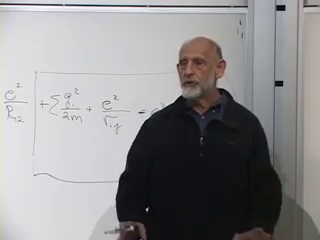
\includegraphics[width=0.72\textwidth]{lecture_01_figure_02.png}
\caption{Молекулярный гамильтониан остается на доске, пока вводится задача об основном состоянии электронной подсистемы. Набранная форма в формуле~\eqref{eq:molecular-hamiltonian} фиксирует члены, скрытые в этом кадре.}
\lectureframe{00:16:19}
\end{figure}

\begin{classroomqa}
\audiencequestion{Ядерные импульсы просто приравниваются нулю?\lecturetimestamp{00:15:39}}
\lecturerresponse{Только временно. В ведущем приближении ядра считаются как бы жестко закрепленными, потому что они движутся намного медленнее электронов. Их импульсы будут восстановлены, когда мы будем решать эффективную задачу для ядер, так что это приближение не нарушает принцип неопределенности.}
\end{classroomqa}

Энергия основного электронного состояния теперь дает вклад в потенциал, который ощущают ядра:
\begin{equation}
V_{\mathrm{eff}}(R_1,R_2)
=\frac{e^2}{R_{12}}+E_{\mathrm{el}}(R_1,R_2).
\label{eq:molecular-effective-potential}
\end{equation}
Для двух изолированных атомов вращательная и трансляционная инвариантность сводят его к функции от расстояния между ними \(R_{12}\). На очень малых расстояниях доминирует кулоновское отталкивание ядер. На очень больших расстояниях взаимодействие слабо. Между этими пределами электронное облако может создать область притяжения и минимум. Тогда волновая функция ядер локализуется вблизи этого минимума и описывает связанную молекулу.

Обратите внимание на порядок действий. Мы не угадывали эмпирическое притяжение и не выбрасывали электроны. Сначала мы решили их квантовую задачу на фиксированном ядерном фоне. Лишь затем мы стерли их явные координаты и сохранили полученное собственное значение. Физика коротких расстояний сохраняется в форме, глубине и кривизне \(V_{\mathrm{eff}}\). Положение его минимума задает равновесное расстояние, его кривизна управляет малыми колебаниями, а его асимптотическая форма определяет, существует ли связанное состояние. Одна эффективная функция переносит всю эту электронную информацию в более медленную задачу.

Таким образом, сложный многоэлектронный гамильтониан превратился в двухчастичный гамильтониан ядер с новым потенциалом. Мы устранили быстрые степени свободы, но сохранили весь их низкоэнергетический эффект. Потенциал ренормирован. Это знакомое рассуждение Борна--Оппенгеймера обычно не вводят под таким названием, однако в нем содержится в точности нужная нам идея:
\begin{equation}
\begin{gathered}
\text{fast microscopic dynamics}\\
\Downarrow\\
\text{effective parameters for slow dynamics}
\end{gathered}
\end{equation}

\section{Естественные единицы и размерность поля}

В квантовой теории поля устраняемые моды можно равносильно описывать как моды коротких расстояний, коротких длин волн, высоких частот или высоких энергий. Прежде чем рисовать диаграммы, зафиксируем учет размерностей.

В обычной механике используются независимые единицы длины, времени и массы. В физике элементарных частиц полагают
\begin{equation}
\hbar=c=1.
\end{equation}
Тогда энергия и масса эквивалентны благодаря \(E=mc^2\), длина и время эквивалентны, потому что \(c=1\), а благодаря \(\hbar=1\) импульс имеет размерность обратной длины. Остается только одна размерность:
\begin{equation}
[M]=[E]=[p]=L^{-1},
\qquad
[x]=[t]=L.
\label{eq:natural-units}
\end{equation}

Это не отменяет размерностей. Просто выбираются коэффициенты пересчета так, что время можно выражать как длину, а массу — как обратную длину. Как только задана одна единица, все остальные определяются автоматически. Поэтому обрезание можно описывать либо как малое расстояние \(\delta\), либо как высокую энергию
\(\Lambda=1/\delta\): это один и тот же масштаб, выраженный на двух языках.

Рассмотрим одно вещественное скалярное поле \(\phi\) со схематически нормированной плотностью лагранжиана
\begin{equation}
\mathcal L=(\partial_\mu\phi)(\partial^\mu\phi)-V(\phi),
\qquad
S=\int d^4x\,\mathcal L.
\label{eq:scalar-action}
\end{equation}

\begin{figure}[htbp]
\centering
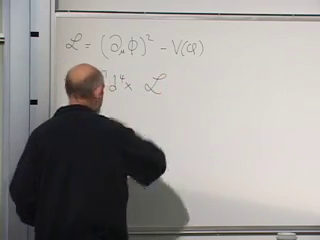
\includegraphics[width=0.78\textwidth]{lecture_01_figure_03.png}
\caption{Локальная скалярная плотность лагранжиана и её интеграл по пространству-времени, образующий действие.}
\lectureframe{00:26:08}
\end{figure}

Плотность лагранжиана локальна: она описывает одну точку пространства-времени. Классические уравнения поля получаются из условия стационарности действия. В квантовой теории то же действие входит в фазу интеграла по траекториям \(\exp(iS)\). В обоих подходах решающей оказывается размерность \(S\). Если восстановить \(\hbar\), фаза имеет вид \(\exp(iS/\hbar)\); после выбора \(\hbar=1\) сама величина \(S\) должна быть безразмерной.

\begin{classroomqa}
\audiencequestion{Имеет ли действие размерность
\(\hbar\)?\lecturetimestamp{00:26:13}}
\lecturerresponse{Да. Поскольку \(\hbar\) положена равной единице, в этих единицах действие безразмерно. Четырёхмерная мера имеет размерность \(L^4\), поэтому плотность лагранжиана должна иметь размерность \(L^{-4}\).}
\end{classroomqa}

Кинетический член теперь фиксирует размерность поля:
\begin{align}
[S]&=1, & [\mathcal L]&=L^{-4},\\
[\partial_\mu]&=L^{-1}, &
[(\partial\phi)^2]&=L^{-2}[\phi]^2=L^{-4},\nonumber\\
&& [\phi]&=L^{-1}.
\label{eq:scalar-dimension}
\end{align}
Этот небольшой расчёт определит ультрафиолетовый порядок величины каждой диаграммы, которая появится далее.

Разложим потенциал в виде
\begin{equation}
V(\phi)=\frac{m^2}{2}\phi^2+g\phi^3+\lambda\phi^4+\cdots.
\label{eq:scalar-potential}
\end{equation}
Каждый член должен иметь размерность \(L^{-4}\). Поскольку
\([\phi^n]=L^{-n}\),
\begin{equation}
[m^2]=L^{-2},
\qquad
[g]=L^{-1},
\qquad
[\lambda]=1.
\label{eq:coupling-dimensions}
\end{equation}
Константа квартического взаимодействия безразмерна. Такие константы связи особенно важны при перенормировке, поскольку их зависимость от масштаба не выводится из простой степени длины.

\begin{classroomqa}
\audiencequestion{Имеет ли \(g\) размерность массы?\lecturetimestamp{00:29:52}}
\lecturerresponse{Да. Множитель \(\phi^3\) имеет размерность \(L^{-3}\), тогда как плотность потенциала должна иметь размерность \(L^{-4}\). Следовательно, \([g]=L^{-1}\), что в естественных единицах соответствует массе.}
\end{classroomqa}

\section{Вершины и пропагатор на коротких расстояниях}

Правила Фейнмана строятся из вершин и пропагаторов. Член \(g\phi^3\) даёт вершину с тремя линиями, которой соответствует множитель, пропорциональный \(g\); \(\lambda\phi^4\) даёт вершину с четырьмя линиями, которой соответствует множитель, пропорциональный \(\lambda\). Квадратичный член даёт локальную двухточечную вставку. Её можно изобразить как частицу, которая входит, поглощается и вновь испускается, с коэффициентом, пропорциональным \(m^2/2\). Численные нормировки, знаки, множители \(i\) и факторы симметрии намеренно опущены, потому что в лекции извлекают зависимость от масштаба, а не вычисляют сечение.

У этих рисунков есть операционное прочтение. Трёхточечная вершина может поглотить два кванта и испустить один, либо представлять любое связанное с кроссингом назначение её трёх линий. Четырёхточечная вершина может описывать две входящие и две выходящие частицы. Квадратичный крестик всё ещё является допустимой двухлинейной вершиной, хотя обычно его включают в свободный пропагатор. Мы изображаем его явно, потому что всякий неразрешённый двухточечный процесс вскоре будет распознаваться сравнением с ним.

Пропагатор соединяет две точки пространства-времени. Его линия не означает, что квантовая частица следовала по прямолинейной классической траектории. Она представляет амплитуду создать возбуждение поля в \(x\) и уничтожить или зарегистрировать его в \(y\):
\begin{equation}
\Delta(x-y)=\langle0|\phi(y)\phi(x)|0\rangle.
\label{eq:position-propagator}
\end{equation}
Читайте это выражение справа налево. Действие \(\phi(x)\) на вакуум создаёт одночастичную компоненту в \(x\). Действие \(\phi(y)\) на бра-вектор уничтожает компоненту в \(y\). Их вакуумный матричный элемент есть амплитуда перекрытия между созданием в первой точке и регистрацией во второй. Символы \(x\) и \(y\) обозначают целые четырёхвекторы, а не только две декартовы координаты.

Состояния не имеют физической размерности, тогда как каждое поле имеет размерность \(L^{-1}\). Следовательно,
\begin{equation}
[\Delta]=L^{-2}.
\end{equation}
Для безмассового поля внутреннего масштаба длины нет, и размерный анализ вынуждает короткодистанционное поведение
\begin{equation}
\Delta(x-y)\sim\frac{1}{(x-y)^2}.
\label{eq:massless-propagator}
\end{equation}
В знаменателе стоит лоренц-инвариантный квадрат интервала, с обычным предписанием, необходимым в его сингулярностях.\editorialnote{Для подсчёта степеней удобно выполнить поворот Вика к евклидову разделению, где величина однозначно пропорциональна \(1/|x-y|^2\). Это не меняет ультрафиолетовые степени, используемые ниже.}

Когда \(y\) приближается к \(x\), пропагатор расходится. Эта сингулярность распространения на исчезающе малом интервале является источником, из которого строятся ультрафиолетовые расходимости в более сложных диаграммах.

\section{Как перенормируется масса скалярного поля}

Для скалярного поля динамическим параметром служит \(m^2\), как уже подсказывает релятивистское дисперсионное соотношение:
\begin{equation}
E=\sqrt{\mathbf p^2+m^2}.
\end{equation}
Пусть \(\delta\) — наименьшее расстояние, которое различает наше эффективное описание. Мы не будем различать процессы, вершины которых разделены расстоянием меньше \(\delta\). Любой такой неразрешённый процесс с одним входящим и одним исходящим скаляром имеет ту же наблюдаемую двухточечную структуру, что и массовая вставка, и потому должен вносить вклад в эффективную массу.

Рассматривайте ускоритель как микроскоп. Если его предельное разрешение равно \(\delta\), то поглощение в одной точке, за которым следует испускание на расстоянии, намного меньшем \(\delta\), нельзя отличить от действительно локального события. Мы намеренно размываем вершину на этом масштабе. Перенормировка — это правило, которое переносит все такие альтернативы ниже предела разрешения в коэффициент соответствующего локального оператора.

\subsection{Первая поправка от квартического взаимодействия}

Начнём с одной вершины \(\phi^4\). Две линии относятся к внешней частице; две другие замыкаются в короткую петлю, испускаемую и вновь поглощаемую почти в одной и той же точке. Если размазать пропагатор в совпадающих точках по расстоянию отсечки, получаем
\begin{equation}
\Delta(0)\ \longrightarrow\ \Delta(\delta)\sim\frac{1}{\delta^2},
\end{equation}
и, следовательно,
\begin{equation}
\delta m^2_{(1)}\sim\frac{\lambda}{\delta^2}.
\label{eq:one-loop-scalar-mass}
\end{equation}
Если \(m_0^2\) обозначает исходный, или голый, параметр, то коэффициент двухточечного члена при низком разрешении схематически имеет вид
\begin{equation}
\frac{m_{\mathrm{eff}}^2}{2}
\sim
\frac{m_0^2}{2}
+c_1\frac{\lambda}{\delta^2},
\label{eq:first-renormalized-mass}
\end{equation}
где \(c_1\) включает в себя опущенные численные и зависящие от соглашений множители. Лабораторная масса, измеряемая в экспериментах, которые не разрешают расстояния меньше \(\delta\), — это именно эта перенормированная величина, а не одно лишь \(m_0\).

Итак, наблюдаемое двухточечное событие может происходить двумя неразличимыми способами. Исходная квадратичная вершина может поглотить и вновь испустить частицу, либо квартическое взаимодействие может сделать то же самое, кратковременно испустив и вновь поглотив виртуальный скаляр. Квантовая механика складывает амплитуды. Как только петля оказывается ниже масштаба разрешения, её отдельная история исчезает из эффективного описания, но её вклад в измеряемый коэффициент — нет.

\subsection{Следующая поправка от квартического взаимодействия}

Теперь соединим две квартические вершины так, чтобы одна внешняя частица входила в \(x\), одна выходила из \(x+\Delta\), а три внутренних пропагатора соединяли вершины. Возникают две степени \(\lambda\), а пропагаторы дают \(\Delta^{-6}\). Квантовые амплитуды нужно просуммировать по всем неразрешённым точкам, из которых может выйти исходящая частица, поэтому интегрирование ведётся по относительному четырёхвектору:
\begin{equation}
\delta m^2_{(2)}
\sim
\lambda^2
\int_{|\Delta|\gtrsim\delta}
d^4\Delta\,\frac{1}{|\Delta|^6}.
\label{eq:two-loop-power-count}
\end{equation}

\begin{classroomqa}
\audiencequestion{Означает ли маленькая метка у вершины, что там есть только три частицы?\lecturetimestamp{00:46:35}}
\lecturerresponse{Нет. Мы по-прежнему используем квартическое взаимодействие. В каждой вершине сходятся четыре линии; в этой двухточечной диаграмме одна линия внешняя, а три идут между двумя вершинами. Во второй вершине снова сходятся четыре линии.}
\end{classroomqa}

Мера даёт четыре степени длины, а три пропагатора — степень минус шесть. Поскольку в этой оценке единственным масштабом служит ультрафиолетовая отсечка,
\begin{equation}
\int_{|\Delta|\gtrsim\delta}
\frac{d^4\Delta}{|\Delta|^6}
\sim\frac{1}{\delta^2},
\qquad
\delta m^2_{(2)}
\sim\frac{\lambda^2}{\delta^2}.
\label{eq:two-loop-scalar-mass}
\end{equation}
Здесь \(\Delta^\mu\) — четырёхкомпонентная переменная интегрирования; интегрирование ведётся по её временной и трём пространственным компонентам. Строчная \(\delta\) обозначает фиксированную отсечку. В лекции сначала для обеих величин употребляется одно и то же произносимое название, а позже обозначения уточняются.

Тот же результат виден, если записать четырёхмерную меру в радиальных координатах. С точностью до углового множителя,
\begin{equation}
\int_{\delta}\frac{d^4\Delta}{|\Delta|^6}
\sim
\int_{\delta}\frac{R^3\,dR}{R^6}
=\int_{\delta}\frac{dR}{R^3}
\sim\frac{1}{\delta^2}.
\end{equation}
Именно поэтому верхний предел на больших расстояниях несуществен для ультрафиолетовой оценки: интеграл определяется своим нижним пределом.

В диаграммах более высокого порядка эта схема повторяется. Диаграмма с большим числом квартических вершин вносит более высокую степень \(\lambda\), но размерный анализ по-прежнему допускает квадратично расходящийся вклад в массу:
\begin{equation}
\begin{aligned}
m_{\mathrm{eff}}^2
={}&m_0^2
+\frac{1}{\delta^2}
\left(c_1\lambda+c_2\lambda^2+c_3\lambda^3+\cdots\right)\\
&+\text{weaker terms}.
\end{aligned}
\label{eq:scalar-mass-series}
\end{equation}

\subsection{Кубическое взаимодействие и логарифм}

Две кубические вершины дают два пропагатора между близкими точками. Их вклад ведёт себя как
\begin{equation}
\delta m_g^2
\sim
g^2\int_{|\Delta|\gtrsim\delta}
\frac{d^4\Delta}{|\Delta|^4}.
\label{eq:cubic-loop}
\end{equation}
Теперь в мере и знаменателе стоят одинаковые степени. Оставшаяся зависимость логарифмическая, а не степенная:
\begin{equation}
\delta m_g^2
\sim
c_g g^2\log\!\left(\frac{1}{\mu\delta}\right).
\label{eq:cubic-log}
\end{equation}
Масштаб сравнения \(\mu\) делает логарифм безразмерным. Это полностью размерная запись схематического \(g^2\log\delta\) из лекции. Логарифм меняется гораздо медленнее любой обратной степени, поэтому при уменьшении длины отсечки доминирует \(1/\delta^2\).

И здесь радиальная форма снова делает различие наглядным:
\begin{equation}
\int_{\delta}^{R_{\mathrm{IR}}}
\frac{d^4\Delta}{|\Delta|^4}
\sim
\int_{\delta}^{R_{\mathrm{IR}}}\frac{R^3\,dR}{R^4}
=\log\!\left(\frac{R_{\mathrm{IR}}}{\delta}\right).
\end{equation}
Равные степени в мере и знаменателе дают логарифм. Большее число степеней в знаменателе даёт обратную степень отсечки. Лекция не требует от нас вычислять угловые множители; она учит нас с первого взгляда распознавать ультрафиолетовый ответ.

\begin{classroomqa}
\audiencequestion{Какое основание у логарифма?\lecturetimestamp{00:57:42}}
\lecturerresponse{Используйте натуральный логарифм. Смена основания лишь умножает его на числовую константу, и эта константа поглощается тем коэффициентом, для которого множители \(2\), \(\pi\) и симметрийные множители здесь не вычислялись.}
\end{classroomqa}

\begin{classroomqa}
\audiencequestion{Как можно брать логарифм от длины и откуда берётся размерность поправки к массе?\lecturetimestamp{00:58:32}}
\lecturerresponse{Логарифм всегда сопоставляет два масштаба; строго говоря, это логарифм безразмерного отношения, такого как \(1/(\mu\delta)\). Константа связи \(g\) имеет размерность массы в первой степени, так что \(g^2\) уже имеет в точности размерность квадрата массы, которая и требуется для этой поправки.}
\end{classroomqa}

\begin{classroomqa}
\audiencequestion{Диаграмма Фейнмана даёт амплитуду. Является ли квадрат её модуля вероятностью?\lecturetimestamp{00:59:41}}
\lecturerresponse{Да, когда амплитуду подставляют в расчёт физического перехода с необходимыми факторами состояний и фазового пространства. Здесь её более непосредственная роль иная: неразрешённая двухточечная амплитуда имеет ту же локальную форму, что и массовый член, и потому сдвигает эффективный параметр массы.}
\end{classroomqa}

\section{Каждый параметр становится эффективным}

Бесконечное семейство массовых диаграмм не исчезает просто потому, что \(\lambda\) мало. Теория возмущений упорядочивает их по степеням константы связи, так что последующие члены могут становиться меньше, но их всё равно бесконечно много. То же исключение короткодистанционных вкладов перенормирует и сами взаимодействия.

\begin{classroomqa}
\audiencequestion{Даже для перенормировки массы разве диаграмм не бесконечно много?\lecturetimestamp{01:00:35}}
\lecturerresponse{Да. Если \(\lambda\) достаточно мало, ряд теории возмущений может быть полезен, потому что всё более высокие степени последовательно подавляются. Тем не менее перенормированный параметр определяется всем рядом, а не одним лишь первым рисунком.}
\end{classroomqa}

Операционально локальное взаимодействие \(\lambda\phi^4\) — это амплитуда процесса с двумя частицами на входе и двумя на выходе. Если более сложный четырёхточечный процесс целиком происходит внутри неразрешаемой области, то при низком разрешении он неотличим от исходной локальной вершины. Поэтому такие диаграммы объединяются в эффективную \(\lambda\). Их ведущая зависимость от масштаба в четырёхмерной теории \(\phi^4\) обычно логарифмическая. В лекции эта бета-функция не вычисляется; этот пример используется, чтобы сформулировать общее утверждение:
\begin{equation}
\begin{gathered}
\text{parameters measured at low energy}\\
\ne\\
\text{parameters entered at the microscopic cutoff}
\end{gathered}
\end{equation}

Этот четырёхточечный пример важен, потому что устраняет возможное недоразумение. Перенормировка — не специальное исправление, применяемое только к расходимости массы. Каждый оператор, допустимый в лагранжиане, может быть воспроизведён неразрешёнными диаграммами с теми же внешними линиями и симметриями. Двухточечный процесс перенормирует коэффициент при квадратичном члене, четырёхточечный процесс перенормирует коэффициент при члене четвёртой степени, а процессы из вакуума в вакуум будут перенормировать постоянный член. Низкоэнергетический лагранжиан — это компактный реестр, в котором записаны все эти короткодистанционные процессы.

\begin{classroomqa}
\audiencequestion{Поскольку \(\Delta\) имеет размерность длины, разве логарифм от неё не выглядит размерностно странно? И разве на доске не перепутали прописную и строчную дельту?\lecturetimestamp{01:01:34}}
\lecturerresponse{Логарифм на самом деле означает отношение к другому масштабу и потому безразмерен. Да, обозначения на мгновение были перепутаны: \(\Delta^\mu\) — переменная интегрирования, а \(\delta\) — нижнее отсечение по расстоянию, которое остаётся в ответе.}
\end{classroomqa}

Это полетеоретический аналог случая с молекулой. Мы решили задачу для ненаблюдаемых быстрых электронов и включили их результат в потенциал. Здесь мы суммируем ненаблюдаемые короткодистанционные процессы и включаем их результат в массы, константы связи и все остальные допустимые локальные коэффициенты. Сдвигается всё.

\begin{classroomqa}
\audiencequestion{Не могли бы вы повторить: включает ли измеряемая величина масштабы, меньшие тех, которые эксперимент способен увидеть?\lecturetimestamp{01:05:13}}
\lecturerresponse{Да, включает. Их отдельные флуктуации не разрешаются, но их суммарный эффект присутствует. Все диаграммы, включающие более короткие масштабы, собираются в один эффективный коэффициент, который низкоэнергетический эксперимент называет, например, физическим квадратом массы.}
\end{classroomqa}

\begin{classroomqa}
\audiencequestion{Должен ли тогда исходный член \(m_0^2\) компенсировать остальные вклады?\lecturetimestamp{01:06:00}}
\lecturerresponse{Если измеряемая масса скаляра намного меньше отдельных ультрафиолетовых вкладов, то да. Требуемая компенсация и есть проблема тонкой настройки, к которой мы теперь переходим.}
\end{classroomqa}

\section{Проблема иерархии Хиггса}

Представьте, что отсечение задаётся планковской длиной, так что от эффективной теории поля требуется суммировать флуктуации от лабораторных масштабов вплоть до масштаба, на котором должна вступить квантовая гравитация.
В единицах физики частиц,
\begin{equation}
\delta\sim M_{\mathrm{Pl}}^{-1}\sim10^{-19}\,\mathrm{GeV}^{-1},
\qquad
\frac{1}{\delta^2}\sim10^{38}\,\mathrm{GeV}^2.
\label{eq:planck-cutoff}
\end{equation}
Точное использование приведённого или неприведённого масштаба Планка несущественно для этого огромного сравнения.

Иерархия расстояний столь же поразительна. Планковская длина примерно на девятнадцать порядков меньше радиуса протона и примерно на шестнадцать или семнадцать порядков меньше расстояний, непосредственно зондируемых обсуждаемыми ускорителями. Именно возведение этого отношения в квадрат превращает большую иерархию длин в компенсацию примерно до 34-го знака после запятой в параметре квадрата массы скаляра.

Для поля Хиггса, скаляра, желаемый слабый масштаб имеет порядок нескольких сотен ГэВ, а не \(10^{19}\) ГэВ. Однако члены в уравнении ~\eqref{eq:scalar-mass-series} естественным образом могут иметь величину планковского масштаба. Их знаки здесь не отслеживались: некоторые могут быть положительными, а некоторые отрицательными, и голый параметр квадрата массы тоже может иметь любой знак. Но чтобы остался остаток электрослабого масштаба, эти огромные части должны сократиться примерно до 34-го знака после запятой. Сначала Susskind говорит о 17 знаках, а затем исправляет себя, потому что сравнение идёт между квадратами масс. Именно квадрат отношения и измеряет эту разновидность тонкой настройки.

\begin{classroomqa}
\audiencequestion{\(\lambda\) меньше или больше единицы?\lecturetimestamp{01:09:50}}
\lecturerresponse{Предполагается, что она умеренно меньше единицы. Теория возмущений стала бы неуправляемой, если бы последовательные степени росли, а чисто скалярную теорию также нельзя согласованно экстраполировать при сколь угодно большой квартической константе связи. Но \(\lambda\) и близко не столь мало, как \(10^{-38}\); для ориентировки в лекции берётся число порядка процентов.}
\end{classroomqa}

\begin{classroomqa}
\audiencequestion{Даже если \(\lambda<1\), разве не остаются важными многие члены, поскольку каждый несёт большой фактор отсечения?\lecturetimestamp{01:10:43}}
\lecturerresponse{Да. Более высокие степени в конце концов подавляют ряд, но до этого заметный вклад может дать большое число членов. Им всем вместе с голым членом пришлось бы согласованно подстроиться, чтобы оставить необычайно малый физический результат.}
\end{classroomqa}

Напомним, почему известно, что параметр массы Хиггса имеет электрослабый масштаб. В обозначениях лекции потенциал нарушения симметрии записывается как
\begin{equation}
V(\phi)=-\frac{\mu^2}{2}\phi^2+\frac{\lambda}{4}\phi^4.
\label{eq:higgs-potential}
\end{equation}
Отрицательный коэффициент при квадратичном члене делает начало координат неустойчивым, тогда как положительный квартический член стабилизирует потенциал. Дифференцирование,
\begin{equation}
\frac{dV}{d\phi}=-\mu^2\phi+\lambda\phi^3
=\phi(-\mu^2+\lambda\phi^2),
\end{equation}
даёт ненулевой минимум
\begin{equation}
\phi_{\min}^2=f^2=\frac{\mu^2}{\lambda}.
\label{eq:higgs-minimum}
\end{equation}
На доске квартический член схематически записан как \(\lambda\phi^4\), но цитируется уравнение ~\eqref{eq:higgs-minimum}; вставка обычного множителя \(1/4\) делает эти две строки согласованными, не меняя аргумента.

Знак \(-\mu^2\) важен, но не спасает естественность. Именно отрицательная кривизна в начале координат приводит к спонтанному нарушению симметрии. Перенормировка сдвигает эту кривизну большими положительными и отрицательными вкладами. Наблюдаемый вакуум с нарушенной симметрией требует, чтобы их сумма была не просто малой, а имела то конкретное малое отрицательное значение, которое помещает минимум на электрослабый масштаб.

Массы бозонов \(W\) и \(Z\) определяют \(f\) как величину порядка \(200\,\mathrm{GeV}\) в грубой нормировке, используемой в лекции. Если \(\lambda\) не является ни огромной, ни фантастически малой, то \(\mu\) должен иметь тот же общий порядок. Следовательно, наблюдаемый коэффициент электрослабого масштаба есть остаток вкладов, каждый из которых может быть на многие десятки порядков больше.

Это называют проблемой тонкой настройки Хиггса, проблемой иерархии или проблемой калибровочной иерархии. Иерархия — это громадное отношение между обычным слабым масштабом и возможным масштабом объединения или планковским масштабом. Малое число само по себе не обязано быть парадоксом. Тревожит здесь то, что малое число собрано из больших, по-видимому не связанных между собой частей, которые должны компенсировать друг друга с чрезвычайной точностью. Эта проблема была осознана в конце 1970-х и начале 1980-х годов, и поиск механизма, стоящего за такой компенсацией, служит мотивацией для суперсимметрии и ряда конкурирующих идей.

Бесконечный ряд теории возмущений не снимает проблему, а лишь обостряет её. \(\lambda\) порядка процентов делает достаточно высокие степени малыми, но прежде чем это подавление начнёт преобладать, может накопиться много членов. Недостаточно, чтобы однопетлевой вклад случайно сократил голую массу. Эффективный слабый масштаб должен оставаться устойчивым и после учёта остальных короткодистанционных процессов. Объяснением было бы структурное соотношение между членами; несвязанная компенсация цифра за цифрой — всего лишь подстройка.

\section{Почему масса фермиона ведёт себя лучше}

Другие частицы Стандартной модели не требуют независимых подстроек того же рода. Для дираковского фермиона массовый член имеет вид
\begin{equation}
\mathcal L_m=-m\bar\psi\psi
=-m\left(\bar\psi_L\psi_R+\bar\psi_R\psi_L\right).
\label{eq:fermion-mass}
\end{equation}
Он содержит саму массу, а не её квадрат, и связывает левую и правую хиральности. Поэтому локальная массовая вставка переводит \(L\) в \(R\) или \(R\) в \(L\).

\begin{figure}[htbp]
\centering
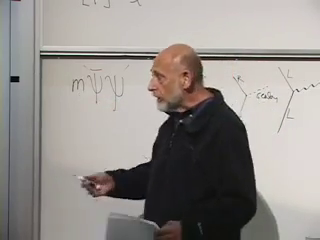
\includegraphics[width=0.76\textwidth]{lecture_01_figure_04.png}
\caption{Фермионный массовый член и нарисованные на доске схематические линии, меняющие хиральность. Ниже диаграммы восстановлены алгебраически, поскольку часть мелового рисунка заслонена.}
\lectureframe{01:23:36}
\end{figure}

В устной лекции часто говорится о лево- или праворукости либо о спиральности. Точную формулировку защиты удобнее всего давать в терминах хиральности. Для ультрарелятивистской частицы картина в терминах спиральности даёт нужную интуицию, но хиральность — это именно та величина, которую несут лево- и правохиральные поля в Eq.~\eqref{eq:fermion-mass}.

Калибровочные взаимодействия сохраняют хиральность:
\begin{equation}
L\xrightarrow{\ \gamma\ }L,
\qquad
R\xrightarrow{\ \gamma\ }R.
\label{eq:gauge-preserves-chirality}
\end{equation}
Юкавское взаимодействие со скаляром соединяет противоположные хиральности:
\begin{equation}
L\xleftrightarrow{\ \phi\ }R.
\label{eq:scalar-flips-chirality}
\end{equation}
Предположим сначала, что у электрона \(m_0=0\). Испускание и повторное поглощение любого числа фотонов не может породить массу, потому что каждая калибровочная вершина сохраняет хиральность. Последовательность, начинающаяся слева, остаётся левой. Поэтому чистая квантовая электродинамика вполне согласованно допускает безмассовый электрон: его электромагнитная собственная энергия не может создать аддитивную массу из нуля.

На языке линий начнём с левохирального электрона. В первой фотонной вершине он всё ещё левохирален; после распространения и повторного поглощения фотона он всё ещё левохирален. Повторение этой конструкции лишь добавляет новые вершины, сохраняющие хиральность. Внешняя двухточечная функция может перенормироваться, но приобрести лево-правую структуру, определяющую массу, она не может.

Может ли это сделать испускание скаляра? Одна скалярная вершина переводит \(L\) в \(R\), но испущенный скаляр должен быть затем поглощён. Поэтому двухточечная диаграмма собственной энергии содержит чётное число скалярных вершин. Второй переворот отменяет первый, так что полная диаграмма снова сохраняет внешнюю хиральность. Как бы ни усложнялась внутренняя диаграмма, испускание и поглощение попарно связывают вершины и не дают появиться аддитивному члену, соединяющему \(L\) и \(R\), когда исходная масса равна нулю.

Это аргумент о чётности числа переворотов. Одна скалярная вершина один раз переворачивает хиральность; замыкание каждой внутренней скалярной линии требует второго конца и, следовательно, второго переворота. Четыре скалярные вершины переворачивают её четырежды и так далее. Чётное число возвращает фермион к исходной хиральности. Вывод не ограничивается простейшей петлёй, нарисованной на доске.

Ненулевая поправка к массе становится возможной только тогда, когда диаграмма уже содержит массовую вставку. Например, испускание и повторное поглощение фотона могут окружать одну вставку \(m_0\bar\psi\psi\). Калибровочные вершины вносят две степени электрического заряда, но единственный переворот хиральности вносит исходную массу:
\begin{equation}
\begin{aligned}
m_e
&=m_0+c_1e^2m_0+c_2e^4m_0+\cdots\\
&=m_0\left(1+c_1e^2+c_2e^4+\cdots\right).
\end{aligned}
\label{eq:multiplicative-fermion-mass}
\end{equation}
Если \(m_0=0\), результат остаётся нулевым. Если \(m_0\) мало, то каждая поправка пропорциональна этой малой величине. Мы всё ещё можем спрашивать, почему электрон лёгок по сравнению с фундаментальным масштабом, но теперь уже не вычитаем огромные несвязанные числа, чтобы его получить. В этом смысле малая масса фермиона технически естественна.

Массовая вставка явно показывает разрешённую последовательность. Начнём с \(L\). Испускание фотона сохраняет \(L\); вставка \(m_0\) переводит \(L\) в \(R\); повторное поглощение фотона сохраняет \(R\). Теперь диаграмма имеет внешнюю хиральность массового члена, но её значение обязательно содержит множитель \(m_0\). В этом и состоит ключевое отличие от Eq.~\eqref{eq:one-loop-scalar-mass}, чья скалярная поправка остаётся ненулевой даже тогда, когда исходная скалярная масса положена равной нулю.

У калибровочных бозонов есть аналогичная защита: калибровочная симметрия запрещает независимый массовый член, поэтому калибровочный бозон, который изначально безмассов, остаётся безмассовым во всех порядках теории возмущений. В Стандартной модели массы фермионов и слабых калибровочных бозонов возникают как следствие среднего значения поля Хиггса. Если масштаб Хиггса взят под контроль, то оставшиеся лёгкие массы не требуют отдельных копий той же катастрофической подстройки.

Тем самым выясняется, на какой вопрос должна отвечать суперсимметрия: может ли теория не допустить, чтобы скаляр Хиггса получил огромную аддитивную поправку к массе? Ответ положителен в должным образом суперсимметричных теориях, потому что бозонные и фермионные вклады связаны между собой, а не независимы. Подробный механизм начинается в следующей лекции.

\section{Другая тонкая подстройка: энергия вакуума}

Есть ещё более серьёзная проблема перенормировки, но наблюдаемой она становится только при учёте гравитации. В негравитационной физике прибавление одной и той же константы ко всем энергиям не меняет ни одного эксперимента. Масса электрона, например, не является абсолютной энергией; это дополнительная энергия, необходимая для добавления электрона к вакууму:
\begin{equation}
m_e=E(\text{vacuum}+\text{one electron})-E(\text{vacuum})
\end{equation}
в системе покоя электрона. Если вакуум и каждое возбуждённое состояние сдвигаются вместе, их разности остаются неизменными.

Тем не менее диаграммы вакуум-вакуум действительно сдвигают энергию вакуума. В теории \(\lambda\phi^4\) соедините четыре ножки одной четырёхточечной вершины в две короткие петли. Каждый пропагатор в совпадающих точках даёт \(1/\delta^2\), так что
\begin{equation}
\delta\rho_{\mathrm{vac}}
\sim
c_{\mathrm{vac}}\frac{\lambda}{\delta^4}.
\label{eq:vacuum-energy-divergence}
\end{equation}
Более сложные вакуумные диаграммы несут другие множители связи и коэффициенты, но размерностный анализ, как правило, оставляет для плотности энергии ту же квартическую зависимость от среза.

Именно отсутствие внешних линий и указывает на эту поправку. Двухточечные диаграммы сравнивают одночастичное состояние с вакуумом и изменяют массу; четырёхточечные изменяют рассеяние; диаграмма без входящих и выходящих частиц изменяет саму амплитуду вакуум-вакуум. Одна четырёхточечная вершина даёт \(\lambda\), а её две короткие петли дают по \(\delta^{-2}\) каждая. Тогда размерностный анализ требует масштаба плотности энергии \(\delta^{-4}\).

Без гравитации можно выбрать аддитивный нуль энергии и спросить: кого это волнует? Общая теория относительности лишает нас этой свободы: тензор энергии-импульса является источником кривизны пространства-времени, так что однородная энергия вакуума заставляет гравитировать само пустое пространство. Она проявляется как космологическая постоянная и наблюдательно связана с тёмной энергией. Тогда малая измеренная энергия вакуума должна сохраняться несмотря на вклады вида \(\delta^{-4}\).

Вот почему при включении гравитации вопрос меняется. В обычной квантовой механике сдвиг всех уровней на одну и ту же константу не затрагивает никаких частот переходов. В гравитации эта константа не является безразличной: тензор энергии-импульса вакуума пропорционален метрике и искривляет пространство-время. То, что было произвольным нулём энергии, становится источником в уравнении Эйнштейна.

Итак, имеются по меньшей мере две крайне острые загадки естественности. В лекции говорится примерно о 123 знаках после запятой для подстройки энергии вакуума и примерно о 30--35 — для подстройки массы Хиггса. Точные оценки зависят от ультрафиолетового масштаба и соглашений, но сам контраст сомнений не вызывает. Суперсимметрия — возможный ответ на обсуждаемую здесь проблему Хиггса; после нарушения суперсимметрии она сама по себе не объясняет наблюдаемую космологическую постоянную.\editorialnote{Вот почему точно суперсимметричная бозон--фермионная компенсация также не является феноменологическим решением проблемы наблюдаемой энергии вакуума: в нашем мире суперсимметрия должна быть нарушена.}

\section{Заключительные вопросы из аудитории}

\begin{classroomqa}
\audiencequestion{Поправка к массе Хиггса зависит от среза \(\delta\), но сам срез кажется произвольным. Может ли это быть планковская длина, десятикратная планковская длина или что-то ещё? Делает ли это тонкую подстройку произвольной?\lecturetimestamp{01:33:50}}
\lecturerresponse{Численный вклад зависит от наименьшего масштаба, до которого эффективной теории ещё доверяют. Эта зависимость — элемент физического учёта, а не уход от проблемы. Моды вплоть до любого масштаба, на котором Стандартная модель всё ещё имеет смысл, — это моды, влияние которых необходимо учитывать. Возьмите \(\delta\) на том расстоянии, где ожидается новая физика---возможно, это планковский масштаб, а возможно, масштаб объединения вблизи \(10^{16}\,\mathrm{GeV}\). Вклад, накопившийся к этому масштабу, уже задаёт нижнюю границу проблемы. Продление той же теории на ещё меньшие расстояния лишь усиливает квадратичную чувствительность. Мы обязаны объяснить, что сокращает вклад от каждого масштаба между лабораторией и этой ультрафиолетовой границей.}
\end{classroomqa}

\begin{classroomqa}
\audiencequestion{Что определяет скалярную частицу и какой можно привести пример?\lecturetimestamp{01:37:26}}
\lecturerresponse{В качестве примера здесь имеется в виду Хиггс. Скаляр при пространственном повороте не преобразуется в разные компоненты; эквивалентно, его кванты имеют нулевой спин. Фотон описывается векторным полем, а гравитационное поле — тензором. На момент этой лекции 2010 года ни одна элементарная частица с нулевым спином еще не была обнаружена.\editorialnote{Бозон Хиггса был открыт в CERN в 2012 году, и его измеренные свойства согласуются с нулевым спином.}}
\end{classroomqa}

\begin{classroomqa}
\audiencequestion{Является ли частица \(Z\) также калибровочным бозоном?\lecturetimestamp{01:38:31}}
\lecturerresponse{Да. \(Z\), \(W^+\) и \(W^-\) — калибровочные бозоны со спином 1, как и фотон. Их уравнения поля и взаимодействия — неабелевы или электрослабые обобщения калибровочного описания типа Максвелла.}
\end{classroomqa}

\begin{classroomqa}
\audiencequestion{Почему бозонный вклад основного состояния не компенсирует фермионный вклад в энергии вакуума?\lecturetimestamp{01:39:10}}
\lecturerresponse{Фермионные петли и соответствующие им бозонные петли действительно могут входить с противоположными знаками. Однако компенсация не происходит автоматически: должны совпадать массы частиц, кратности и константы связи. Даже небольшое несовпадение оставляет значительный остаток, чувствительный к отсечке, и бесконечные семейства диаграмм должны совпадать в каждом порядке. Точная суперсимметрия как раз и обеспечивает такие бозон--фермионные соотношения. Произвольный несуперсимметричный набор частиц этого не обеспечивает, а нарушенная суперсимметрия оставляет остаточную проблему энергии вакуума.}
\end{classroomqa}

\section{Перспектива}

Ход лекции выстроен намеренно. Сначала молекулярный расчет показывает, что исключение быстрых переменных не является ни пренебрежением, ни магией: энергия их основного состояния становится потенциалом для медленных переменных. Квантовая теория поля повторяет эту операцию на разных длинах волн. Затем анализ размерностей показывает, какие эффективные параметры чувствительны к отсечке. Массы скаляров получают аддитивные члены, пропорциональные \(\delta^{-2}\); поэтому малый хиггсовский масштаб кажется неестественно чувствительным. Фермионные массы перенормируются мультипликативно, потому что киральность защищает предел нулевой массы, а калибровочная симметрия аналогичным образом защищает безмассовые калибровочные бозоны. Энергия вакуума еще более чувствительна, масштабируясь как \(\delta^{-4}\), а гравитация делает наблюдаемой ее абсолютную величину.

Суперсимметрия появляется в курсе именно в этот момент не как новое математическое украшение, а как попытка сделать так, чтобы скалярный сектор вел себя больше похоже на защищенные секторы. Следующая задача — понять, какая симметрия может связать бозоны и фермионы достаточно сильно, чтобы организовать эти компенсации.
